\documentclass[12pt, letterpaper]{article}
\usepackage[titletoc,title]{appendix}
\usepackage{color}
\usepackage{booktabs}
\usepackage{caption}
\newcommand\fnote[1]{\captionsetup{font=small}\caption*{#1}}
\usepackage{float}
\usepackage[scaled=.7]{beramono}
\usepackage[usenames,dvipsnames,svgnames,table]{xcolor}
\definecolor{dark-red}{rgb}{0.75,0.10,0.10} 
\usepackage[margin=1in]{geometry}
\usepackage[linkcolor=blue,
            colorlinks=true,
            urlcolor=blue,
            pdfstartview={XYZ null null 1.00},
            pdfpagemode=UseNone,
            citecolor={blue},
            pdftitle={Not News}]{hyperref}

\usepackage{multibib}
\usepackage{geometry} % see geometry.pdf on how to lay out the page. There's lots.
\geometry{letterpaper}               % This is 8.5x11 paper. Options are a4paper or a5paper or other... 
\usepackage{graphicx}                % Handles inclusion of major graphics formats and allows use of 
\usepackage{amsfonts,amssymb,amsbsy}
\usepackage{amsxtra}
\usepackage{natbib}
\usepackage{longtable}
\usepackage{array}
\usepackage{multirow}
\usepackage{wrapfig}
\usepackage{colortbl}
\usepackage{pdflscape}
\usepackage{tabu}
\usepackage{threeparttable}
\usepackage{threeparttablex}
\usepackage[normalem]{ulem}
\usepackage{makecell}
\usepackage{verbatim}
\setcitestyle{round,semicolon,aysep={},yysep={;}}
\usepackage{setspace}             % Permits line spacing control. Options are \doublespacing, \onehalfspace
\usepackage{sectsty}             % Permits control of section header styles
\usepackage{lscape}
\usepackage{fancyhdr}             % Permits header customization. See header section below.
\usepackage{url}                 % Correctly formats URLs with the \url{} tag
\usepackage{fullpage}             %1-inch margins
\usepackage{multirow}
\usepackage{rotating}
\setlength{\parindent}{3em}
\usepackage{subcaption}
\usepackage[T1]{fontenc}
\usepackage{libertine}
\usepackage{inconsolata}
%\usepackage{babel}
\title{\Large{Birthday Voter: Effect of Being Born on Election Day}\footnote{Scripts behind the analysis can be downloaded at: \url{https://github.com/soodoku/birthday_voter}.}}
\author{Jake Leland\thanks{Jake can be reached at \href{mailto:jake.leland@utexas.edu}{\footnotesize{\texttt{jakebleland@gmail.com}}}}
\and Gaurav Sood\thanks{Gaurav can be reached at \href{mailto:gsood07@gmail.com}{\footnotesize{\texttt{gsood07@gmail.com}}}}}

\date{\vspace{.5cm}\normalsize{\today}}

\begin{document}
\maketitle

\begin{comment}

setwd(paste0(githubdir, "birthday_voter/ms"))
tools::texi2dvi("birthday_voter.tex", pdf = TRUE, clean = TRUE) 
setwd(basedir)

\end{comment}

\begin{abstract}

\end{abstract}

\clearpage
\doublespacing
Given the chance of being the pivotal voter is vanishingly small, the cost of voting looms large. Thus, if the aim is to sway policy, it is irrational to turnout \citep{mclean1994condorcet, downs1957economic} (though see \citep{edlin2007voting}). If not to sway policy, why do people vote? \cite{riker1968theory} suggest that people derive some expressive benefits from voting, for instance, utility from fulfilling their duty (see also  \cite{fiorina1976voting}).  And indeed, some data suggests that people vote more because of expressive reasons than instrumental  \citep{kan2001expressive}. In a similar vein, \citep{verba1993citizen} find that income and time do not explain much variation in why people vote.

In this paper, we contribute to the large literature on reasons why people vote. We leverage data on the voting behavior of millions of people to estimate whether people turn out more often if their birthday falls on the voting day. We expect people to vote more often when their birthday falls on the voting day because of three reasons. First, we posit that people see voting as a duty and like doing dutiful things on their birthdays. Second, people may take the day off on their birthdays and use the time to vote. Third, people may be likelier to remember the election day if it falls on their birthday. Given benefit for time should be the same across midterm and presidential election cycles, if time were the key factor, we expect the effect to be: a. similar across midterm and presidential elections (and primary and general elections), b. concentrated among people who vote in-person than mail.
 
Across elections, we find that the average effect of being born on the election day is XX\%. But when we subset on midterm elections, we see an average effect of Y\%. Most of the effect is concentrated in in-person voting, suggesting that memory is less of a factor.

\section{Data and Research Design}
The dataset was extracted as of February 2017 and includes 10 years of elections from 2006 through 2016. There are two files.

\begin{itemize}
	\item \textbf{Official voter registration information}: Data is extracted from the Florida Voter Registration System and includes information on voters who are officially registered or pre-registered as of the end of the prior month. All information is included except limited in those cases in which a voter requested exemption from public disclosure per Section 119.071, Fla. Stat.  (Section 98.0981(1)(b), Fla. Stat.).

	\item \textbf{Unofficial voting history information} Data is extracted from independently submitted reports from the 67 county supervisors of elections capturing voting history at a fixed point in time. 
\end{itemize}

In all, there are X number of voters. 

\subsection{Data Validation}

We apply a set of filters to ensure that only persons at least 18 years old and registered to vote on election day are included in the analysis. We also perform a set of validation checks to confirm the soundness and accuracy of the dataset: 

\begin{itemize}

	\item \textbf{Fake Birthdays}: we search for potential fake birthdays by checking if unusually large proportion of voters' birthdays fall on a specific day.

	\item \textbf{Voter turnout grouped by age}: we expect to see turnout initially go down until people are in college, then increase steadily until about 70-80 years before declining. Figure 1 plots a loess.  

	\item \textbf{Voter turnout during midterms vs. presidential elections}: we expect higher turnout in presidential elections than midterms. We find that the average turnout during presidential elections as YY\% and during the midterms was XX\%. 

	\item \textbf{Voter turnout during general vs. primary elections}: we expect to see higher turnout for general elections than primaries. We find that the average turnout during presidential elections as YY\% and during the primaries was XX\%. 

\end{itemize}

\begin{figure}[H]
\centering
 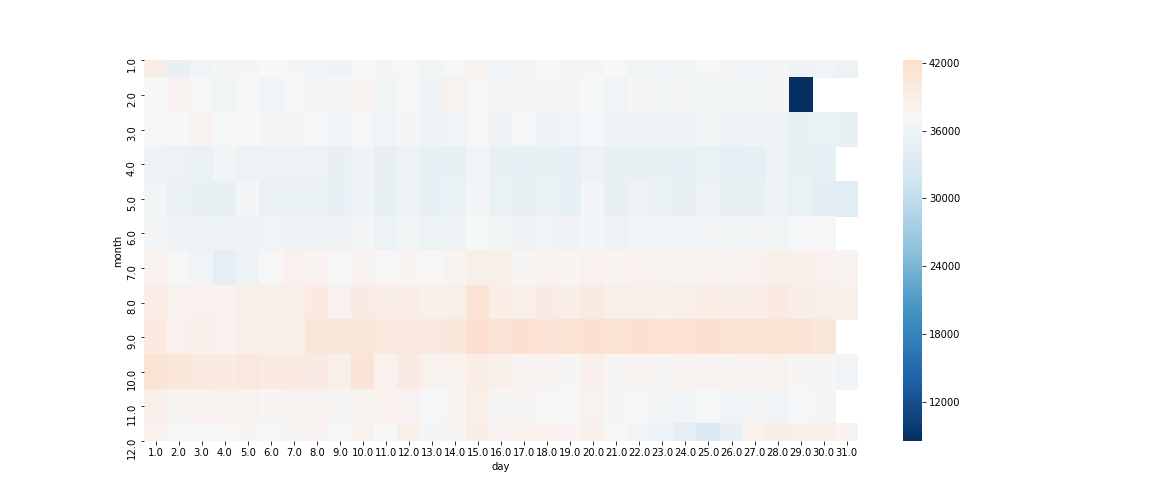
\includegraphics[width=\textwidth]{../figs/fig2_bday_count_by_month_day.png}
 \caption{Birthday Voter}
 \label{fig:birthday}
\end{figure}

The dataset passed the validation checks. For the purposes of this analysis, we also limit the data to primary and general elections receiving at least 100 thousand votes. This leaves us with XX number of observations spanning X mid-term, Y general, and K primary elections. 

% latex table generated in R 4.0.0 by xtable 1.8-4 package
% Tue May 05 23:11:33 2020
\begin{table}[!htb]
\centering
\caption{Effect of Data Quality Filters on the Number of Observations} 
\label{table:filter}
\begingroup\small
\begin{tabular}{lrr}
  \hline
Population & n$\backslash$\_voters & pct$\backslash$\_change \\ 
  \hline
Total\_Voters & 164524296.00 &  \\ 
  After Removing Null Birthdays & 163849416.00 & -0.41 \\ 
  After Removing Non-Registered Voters & 122259442.00 & -25.38 \\ 
  After Removing Voters $<$18 years & 121535401.00 & -0.59 \\ 
  After Removing Voters $>$110 years & 121533388.00 & -0.00 \\ 
   \hline
\end{tabular}
\endgroup
\end{table}

% latex table generated in R 4.0.0 by xtable 1.8-4 package
% Tue May 05 18:08:17 2020
\begin{table}[!htb]
\centering
\caption{Effect of Data Quality Filters on the Number of Observations} 
\label{table:midterm_pres}
\begingroup\small
\begin{tabular}{lrr}
  \hline
Population & n_voters & pct_change \\ 
  \hline
Total_Voters & 164524296.00 &  \\ 
  After Removing Null Birthdays & 163849416.00 & -0.41 \\ 
  After Removing Non-Registered Voters & 122259442.00 & -25.38 \\ 
  After Removing Voters <18 years & 121535401.00 & -0.59 \\ 
  After Removing Voters >110 years & 121533388.00 & -0.00 \\ 
   \hline
\end{tabular}
\endgroup
\end{table}

% latex table generated in R 4.0.0 by xtable 1.8-4 package
% Tue May 05 18:08:17 2020
\begin{table}[!htb]
\centering
\caption{Effect of Data Quality Filters on the Number of Observations} 
\label{table:pri_gen}
\begingroup\small
\begin{tabular}{lr}
  \hline
election_type & prop_voted \\ 
  \hline
GEN & 62.76 \\ 
  PRI & 20.18 \\ 
   \hline
\end{tabular}
\endgroup
\end{table}

% latex table generated in R 4.0.0 by xtable 1.8-4 package
% Tue May 05 23:11:34 2020
\begin{table}[!htb]
\centering
\caption{Summary of Data} 
\label{table:tab4}
\begingroup\small
\begin{tabular}{rlrrr}
  \hline
year & election\_type & election\_date & n\_eligible\_voters & prop\_voted \\ 
  \hline
2006.00 & PRI & 13396.00 & 7351945.00 & 20.85 \\ 
  2006.00 & GEN & 13459.00 & 7438519.00 & 50.32 \\ 
  2008.00 & PRI & 14117.00 & 8339366.00 & 17.96 \\ 
  2008.00 & GEN & 14187.00 & 8720216.00 & 79.73 \\ 
  2010.00 & PRI & 14845.00 & 9299270.00 & 22.47 \\ 
  2010.00 & GEN & 14915.00 & 9402245.00 & 50.58 \\ 
  2012.00 & PRI & 15566.00 & 10330654.00 & 20.50 \\ 
  2012.00 & GEN & 15650.00 & 10725293.00 & 73.33 \\ 
  2014.00 & PRI & 16308.00 & 11619524.00 & 16.88 \\ 
  2014.00 & GEN & 16378.00 & 11760611.00 & 49.16 \\ 
  2016.00 & PRI & 17043.00 & 13084073.00 & 22.26 \\ 
  2016.00 & GEN & 17113.00 & 13461672.00 & 70.61 \\ 
   \hline
\end{tabular}
\endgroup
\end{table}


We get the cartesian product of the voter registration file and the voting history file, such that the primary key of the dataset is $voter_id | election_type | election_date$. We then group by the number of days between the person's birthday and the election date, and calculate the mean voter turnout. We use different windows---30 days, 7 days, 1 days---to estimate the mean difference.

We also compare how the estimate varies by general election, midterms, and primaries, how the effect varies by race. And we explore whether the effect is concentrated among in-person voting than absentee or mail-in ballots.

\section{Results}
The analysis shows a substantial increase in turnout if election day falls on the voter's birthday (see Figure ~\ref{fig:birthday}).

\begin{figure}[H]
\centering
 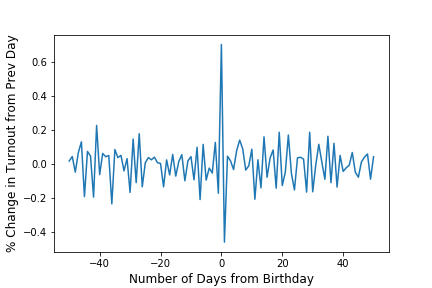
\includegraphics[scale=.7]{../figs/fig1_turnout_chg_from_prev_day.png}
 \caption{Birthday Voter}
 \label{fig:birthday}
\end{figure}

% latex table generated in R 4.0.0 by xtable 1.8-4 package
% Tue May 05 18:08:17 2020
\begin{table}[!htb]
\centering
\caption{Effect of Data Quality Filters on the Number of Observations} 
\label{table:tab5}
\begingroup\small
\begin{tabular}{rrrrr}
  \hline
days_grouped_7 & voted_abs & n_total & n_voters & n_nonvoters \\ 
  \hline
7.00 & 0.35 & 2411271.00 & 997919.00 & 1413352.00 \\ 
  -7.00 & 0.32 & 2409825.00 & 992336.00 & 1417489.00 \\ 
  0.00 & 0.76 & 343829.00 & 143540.00 & 200289.00 \\ 
   \hline
\end{tabular}
\endgroup
\end{table}

% latex table generated in R 4.0.0 by xtable 1.8-4 package
% Tue May 05 23:11:34 2020
\begin{table}[!htb]
\centering
\caption{Effect of Data Quality Filters on the Number of Observations} 
\label{table:tab6}
\begingroup\small
\begin{tabular}{rrrrr}
  \hline
days\_grouped\_30 & voted\_abs & n\_total & n\_voters & n\_nonvoters \\ 
  \hline
-30.00 & 0.30 & 10382628.00 & 4310415.00 & 6072213.00 \\ 
  0.00 & 0.76 & 343829.00 & 143540.00 & 200289.00 \\ 
  30.00 & 0.31 & 10351620.00 & 4251009.00 & 6100611.00 \\ 
   \hline
\end{tabular}
\endgroup
\end{table}

% latex table generated in R 4.0.0 by xtable 1.8-4 package
% Tue May 05 18:08:17 2020
\begin{table}[!htb]
\centering
\caption{Effect of Data Quality Filters on the Number of Observations} 
\label{table:tab7}
\begingroup\small
\begin{tabular}{rrrrr}
  \hline
days_grouped_50 & voted_abs & n_total & n_voters & n_nonvoters \\ 
  \hline
50.00 & 0.31 & 17216272.00 & 7070648.00 & 10145624.00 \\ 
  -50.00 & 0.30 & 17454376.00 & 7323807.00 & 10130569.00 \\ 
  0.00 & 0.76 & 343829.00 & 143540.00 & 200289.00 \\ 
   \hline
\end{tabular}
\endgroup
\end{table}


Tables 1, 2 and 3 show the mean absolute change in turnout for when the election date falls $+/- 50 days,+/-  30 days, and +/- 7$ days from the voter's birthday compared to when the election falls on the voter's birthday. In all three cases, the change in turnout from the previous day is more than two times greater when election date falls on the voter’s birthday.

% latex table generated in R 4.0.0 by xtable 1.8-4 package
% Tue May 05 23:11:34 2020
\begin{table}[!htb]
\centering
\caption{Effect of Data Quality Filters on the Number of Observations} 
\label{table:tab8}
\begingroup\small
\begin{tabular}{rlrrrr}
  \hline
days\_grouped\_7 & race & voted\_abs & n\_total & n\_voters & n\_nonvoters \\ 
  \hline
-7.00 & American Indian or Alaska Native & 5.64 & 7861.00 & 2946.00 & 4915.00 \\ 
  0.00 & American Indian or Alaska Native & 4.02 & 1155.00 & 436.00 & 719.00 \\ 
  7.00 & American Indian or Alaska Native & 4.83 & 7893.00 & 2921.00 & 4972.00 \\ 
  -7.00 & Asian or Pacific Islander & 2.11 & 38004.00 & 12293.00 & 25711.00 \\ 
  0.00 & Asian or Pacific Islander & 1.88 & 5285.00 & 1737.00 & 3548.00 \\ 
  7.00 & Asian or Pacific Islander & 1.80 & 38488.00 & 12316.00 & 26172.00 \\ 
  -7.00 & Black, Not Hispanic & 0.88 & 337163.00 & 128697.00 & 208466.00 \\ 
  0.00 & Black, Not Hispanic & 1.49 & 47915.00 & 18761.00 & 29154.00 \\ 
  7.00 & Black, Not Hispanic & 0.87 & 337584.00 & 128976.00 & 208608.00 \\ 
  -7.00 & Hispanic & 0.65 & 349640.00 & 112321.00 & 237319.00 \\ 
  0.00 & Hispanic & 1.06 & 49647.00 & 16263.00 & 33384.00 \\ 
  7.00 & Hispanic & 0.78 & 351054.00 & 112697.00 & 238357.00 \\ 
  -7.00 & Multi-racial & 4.87 & 10053.00 & 2941.00 & 7112.00 \\ 
  0.00 & Multi-racial & 4.95 & 1472.00 & 456.00 & 1016.00 \\ 
  7.00 & Multi-racial & 4.67 & 10097.00 & 3020.00 & 7077.00 \\ 
  -7.00 & Other & 1.85 & 35984.00 & 11927.00 & 24057.00 \\ 
  0.00 & Other & 1.85 & 5108.00 & 1723.00 & 3385.00 \\ 
  7.00 & Other & 2.65 & 36265.00 & 12356.00 & 23909.00 \\ 
  -7.00 & Unknown & 2.03 & 40122.00 & 11974.00 & 28148.00 \\ 
  0.00 & Unknown & 2.43 & 5618.00 & 1790.00 & 3828.00 \\ 
  7.00 & Unknown & 2.04 & 40202.00 & 12200.00 & 28002.00 \\ 
  -7.00 & White, Not Hispanic & 0.39 & 1590998.00 & 709237.00 & 881761.00 \\ 
  0.00 & White, Not Hispanic & 0.63 & 227629.00 & 102374.00 & 125255.00 \\ 
  7.00 & White, Not Hispanic & 0.40 & 1589688.00 & 713433.00 & 876255.00 \\ 
   \hline
\end{tabular}
\endgroup
\end{table}

% latex table generated in R 4.0.0 by xtable 1.8-4 package
% Tue May 05 18:08:18 2020
\begin{table}[!htb]
\centering
\caption{Effect of Data Quality Filters on the Number of Observations} 
\label{table:tab9}
\begingroup\small
\begin{tabular}{rlrrrr}
  \hline
days_grouped_30 & race & voted_abs & n_total & n_voters & n_nonvoters \\ 
  \hline
30.00 & American Indian or Alaska Native & 5.01 & 33898.00 & 12802.00 & 21096.00 \\ 
  30.00 & Asian or Pacific Islander & 2.06 & 164383.00 & 52176.00 & 112207.00 \\ 
  30.00 & Black, Not Hispanic & 0.84 & 1453661.00 & 552854.00 & 900807.00 \\ 
  30.00 & Hispanic & 0.70 & 1519987.00 & 479916.00 & 1040071.00 \\ 
  30.00 & Multi-racial & 4.33 & 43015.00 & 12840.00 & 30175.00 \\ 
  30.00 & Other & 2.45 & 155479.00 & 52539.00 & 102940.00 \\ 
  30.00 & Unknown & 2.20 & 172960.00 & 52200.00 & 120760.00 \\ 
  30.00 & White, Not Hispanic & 0.38 & 6808237.00 & 3035682.00 & 3772555.00 \\ 
  -30.00 & American Indian or Alaska Native & 5.07 & 34055.00 & 12798.00 & 21257.00 \\ 
  -30.00 & Asian or Pacific Islander & 1.97 & 165686.00 & 53420.00 & 112266.00 \\ 
  -30.00 & Black, Not Hispanic & 0.81 & 1445035.00 & 557657.00 & 887378.00 \\ 
  -30.00 & Hispanic & 0.71 & 1498228.00 & 486371.00 & 1011857.00 \\ 
  -30.00 & Multi-racial & 4.38 & 44690.00 & 13609.00 & 31081.00 \\ 
  -30.00 & Other & 2.06 & 153829.00 & 52022.00 & 101807.00 \\ 
  -30.00 & Unknown & 2.31 & 174234.00 & 53262.00 & 120972.00 \\ 
  -30.00 & White, Not Hispanic & 0.39 & 6866871.00 & 3081276.00 & 3785595.00 \\ 
  0.00 & American Indian or Alaska Native & 4.02 & 1155.00 & 436.00 & 719.00 \\ 
  0.00 & Asian or Pacific Islander & 1.88 & 5285.00 & 1737.00 & 3548.00 \\ 
  0.00 & Black, Not Hispanic & 1.49 & 47915.00 & 18761.00 & 29154.00 \\ 
  0.00 & Hispanic & 1.06 & 49647.00 & 16263.00 & 33384.00 \\ 
  0.00 & Multi-racial & 4.95 & 1472.00 & 456.00 & 1016.00 \\ 
  0.00 & Other & 1.85 & 5108.00 & 1723.00 & 3385.00 \\ 
  0.00 & Unknown & 2.43 & 5618.00 & 1790.00 & 3828.00 \\ 
  0.00 & White, Not Hispanic & 0.63 & 227629.00 & 102374.00 & 125255.00 \\ 
   \hline
\end{tabular}
\endgroup
\end{table}

% latex table generated in R 4.0.0 by xtable 1.8-4 package
% Tue May 05 23:11:35 2020
\begin{table}[!htb]
\centering
\caption{Effect of Data Quality Filters on the Number of Observations} 
\label{table:tab10}
\begingroup\small
\begin{tabular}{rlrrrr}
  \hline
days\_grouped\_50 & race & voted\_abs & n\_total & n\_voters & n\_nonvoters \\ 
  \hline
-50.00 & American Indian or Alaska Native & 4.97 & 57263.00 & 21856.00 & 35407.00 \\ 
  0.00 & American Indian or Alaska Native & 4.02 & 1155.00 & 436.00 & 719.00 \\ 
  50.00 & American Indian or Alaska Native & 4.98 & 55879.00 & 20937.00 & 34942.00 \\ 
  -50.00 & Asian or Pacific Islander & 2.04 & 275798.00 & 89744.00 & 186054.00 \\ 
  0.00 & Asian or Pacific Islander & 1.88 & 5285.00 & 1737.00 & 3548.00 \\ 
  50.00 & Asian or Pacific Islander & 1.99 & 276512.00 & 87371.00 & 189141.00 \\ 
  -50.00 & Black, Not Hispanic & 0.82 & 2407166.00 & 941075.00 & 1466091.00 \\ 
  0.00 & Black, Not Hispanic & 1.49 & 47915.00 & 18761.00 & 29154.00 \\ 
  50.00 & Black, Not Hispanic & 0.82 & 2417340.00 & 924966.00 & 1492374.00 \\ 
  -50.00 & Hispanic & 0.71 & 2516234.00 & 827989.00 & 1688245.00 \\ 
  0.00 & Hispanic & 1.06 & 49647.00 & 16263.00 & 33384.00 \\ 
  50.00 & Hispanic & 0.76 & 2529949.00 & 796775.00 & 1733174.00 \\ 
  -50.00 & Multi-racial & 4.32 & 75303.00 & 23227.00 & 52076.00 \\ 
  0.00 & Multi-racial & 4.95 & 1472.00 & 456.00 & 1016.00 \\ 
  50.00 & Multi-racial & 4.53 & 71484.00 & 21296.00 & 50188.00 \\ 
  -50.00 & Other & 2.14 & 257277.00 & 88073.00 & 169204.00 \\ 
  0.00 & Other & 1.85 & 5108.00 & 1723.00 & 3385.00 \\ 
  50.00 & Other & 2.37 & 258306.00 & 87040.00 & 171266.00 \\ 
  -50.00 & Unknown & 2.22 & 292896.00 & 90442.00 & 202454.00 \\ 
  0.00 & Unknown & 2.43 & 5618.00 & 1790.00 & 3828.00 \\ 
  50.00 & Unknown & 2.13 & 287254.00 & 86779.00 & 200475.00 \\ 
  -50.00 & White, Not Hispanic & 0.37 & 11572439.00 & 5241401.00 & 6331038.00 \\ 
  0.00 & White, Not Hispanic & 0.63 & 227629.00 & 102374.00 & 125255.00 \\ 
  50.00 & White, Not Hispanic & 0.36 & 11319548.00 & 5045484.00 & 6274064.00 \\ 
   \hline
\end{tabular}
\endgroup
\end{table}


% latex table generated in R 4.0.0 by xtable 1.8-4 package
% Tue May 05 18:08:18 2020
\begin{table}[!htb]
\centering
\caption{Effect of Data Quality Filters on the Number of Observations} 
\label{table:tab11}
\begingroup\small
\begin{tabular}{rlrr}
  \hline
days_grouped_7 & history_code & voted_abs & n_voters \\ 
  \hline
7.00 & Absentee & 3.26 & 262702.00 \\ 
  7.00 & Early & 2.95 & 258994.00 \\ 
  7.00 & Polls & 2.06 & 476223.00 \\ 
  -7.00 & Absentee & 3.04 & 262807.00 \\ 
  -7.00 & Early & 4.37 & 254660.00 \\ 
  -7.00 & Polls & 2.43 & 474869.00 \\ 
  0.00 & Absentee & 3.56 & 38230.00 \\ 
  0.00 & Early & 3.36 & 37684.00 \\ 
  0.00 & Polls & 2.97 & 67626.00 \\ 
   \hline
\end{tabular}
\endgroup
\end{table}

% latex table generated in R 4.0.0 by xtable 1.8-4 package
% Tue May 05 18:08:18 2020
\begin{table}[!htb]
\centering
\caption{Effect of Data Quality Filters on the Number of Observations} 
\label{table:tab12}
\begingroup\small
\begin{tabular}{rlrr}
  \hline
days_grouped_30 & history_code & voted_abs & n_voters \\ 
  \hline
30.00 & Absentee & 2.73 & 1113533.00 \\ 
  30.00 & Early & 2.82 & 1098240.00 \\ 
  30.00 & Polls & 2.11 & 2039236.00 \\ 
  -30.00 & Absentee & 3.13 & 1119242.00 \\ 
  -30.00 & Early & 3.59 & 1111925.00 \\ 
  -30.00 & Polls & 2.28 & 2079248.00 \\ 
  0.00 & Absentee & 3.56 & 38230.00 \\ 
  0.00 & Early & 3.36 & 37684.00 \\ 
  0.00 & Polls & 2.97 & 67626.00 \\ 
   \hline
\end{tabular}
\endgroup
\end{table}

% latex table generated in R 4.0.0 by xtable 1.8-4 package
% Tue May 05 18:08:18 2020
\begin{table}[!htb]
\centering
\caption{Effect of Data Quality Filters on the Number of Observations} 
\label{table:tab13}
\begingroup\small
\begin{tabular}{rlrr}
  \hline
days_grouped_50 & history_code & voted_abs & n_voters \\ 
  \hline
50.00 & Absentee & 2.90 & 1851970.00 \\ 
  50.00 & Early & 3.17 & 1826846.00 \\ 
  50.00 & Polls & 2.26 & 3391832.00 \\ 
  -50.00 & Absentee & 3.00 & 1893710.00 \\ 
  -50.00 & Early & 3.47 & 1898768.00 \\ 
  -50.00 & Polls & 2.03 & 3531329.00 \\ 
  0.00 & Absentee & 3.56 & 38230.00 \\ 
  0.00 & Early & 3.36 & 37684.00 \\ 
  0.00 & Polls & 2.97 & 67626.00 \\ 
   \hline
\end{tabular}
\endgroup
\end{table}


\section{Conclusion}
Further research may be warranted to determine the causal relationship between a person's birthday and voting, which may be a result of a sense of duty, having more leisure time, or simply making it easier to remember. Whatever the case may be, our analysis shows that a person is in fact more likely to vote when election day falls on their birthday. 

\clearpage
\bibliographystyle{apsr}
\bibliography{birthday_voter}  

\clearpage
\appendix
\renewcommand{\thesection}{SI \arabic{section}}
\renewcommand\thetable{\thesection.\arabic{table}}  
\renewcommand\thefigure{\thesection.\arabic{figure}}
\counterwithin{figure}{section}

\section{Supporting Information}

\subsection{Supplementary Results}
\begin{figure}[H]
\centering
 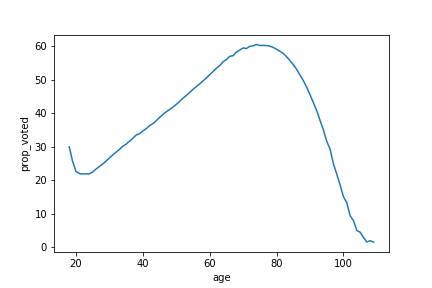
\includegraphics[scale=.7]{../figs/fig3_prop_voted_by_age.png}
 \caption{Birthday Voter}
 \label{fig:birthday}
\end{figure}

\end{document}